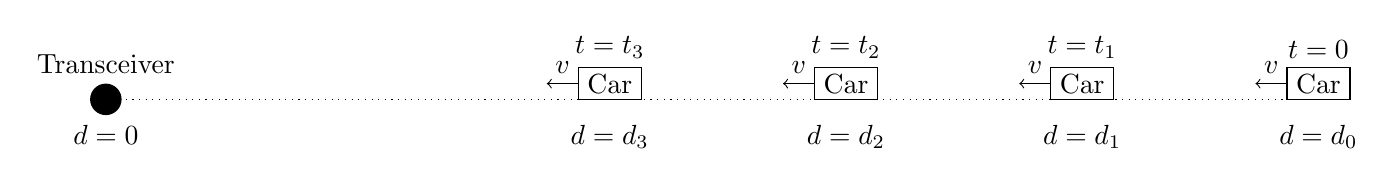
\begin{tikzpicture}

    % Draw the transceiver
    \fill[black] (0,0) circle (0.2) node[above] at (0,0.2) {Transceiver} node[below] at (0,-0.2) {$d=0$};

    % Draw the car at distance D_0
    \draw (15,0) rectangle ++(0.8,0.4) node[midway] {Car} node[above] at (15.4,0.4) {$t=0$ } node[below] at (15.4,-0.2) {$d=d_0$};
    \draw[->] (15,0.2) -- node[above] {$v$} (14.6,0.2);

    \draw (12,0) rectangle ++(0.8,0.4) node[midway] {Car} node[above] at (12.4,0.4) {$t=t_1$ } node[below] at (12.4,-0.2) {$d=d_1$};
    \draw[->] (12,0.2) -- node[above] {$v$} (11.6,0.2);

    \draw (9,0) rectangle ++(0.8,0.4) node[midway] {Car} node[above] at (9.4,0.4) {$t=t_2$ } node[below] at (9.4,-0.2) {$d=d_2$};
    \draw[->] (9,0.2) -- node[above] {$v$} (8.6,0.2);

    \draw (6,0) rectangle ++(0.8,0.4) node[midway] {Car} node[above] at (6.4,0.4) {$t=t_3$ } node[below] at (6.4,-0.2) {$d=d_3$};
    \draw[->] (6,0.2) -- node[above] {$v$} (5.6,0.2);

    \draw[dotted] (0,0) -- (15,0);

\end{tikzpicture}



